\documentclass[12pt]{article}

\usepackage{../thesis}

\usepackage{tikz} 
\usepackage{pgfplots} % drawing plots right here in this file!
\pgfplotsset{compat=1.9} % latest stable release

\begin{document}

\pagestyle{empty}


\begin{tikzpicture}
    \node[anchor=south west,inner sep=0] (image) at (0,0) {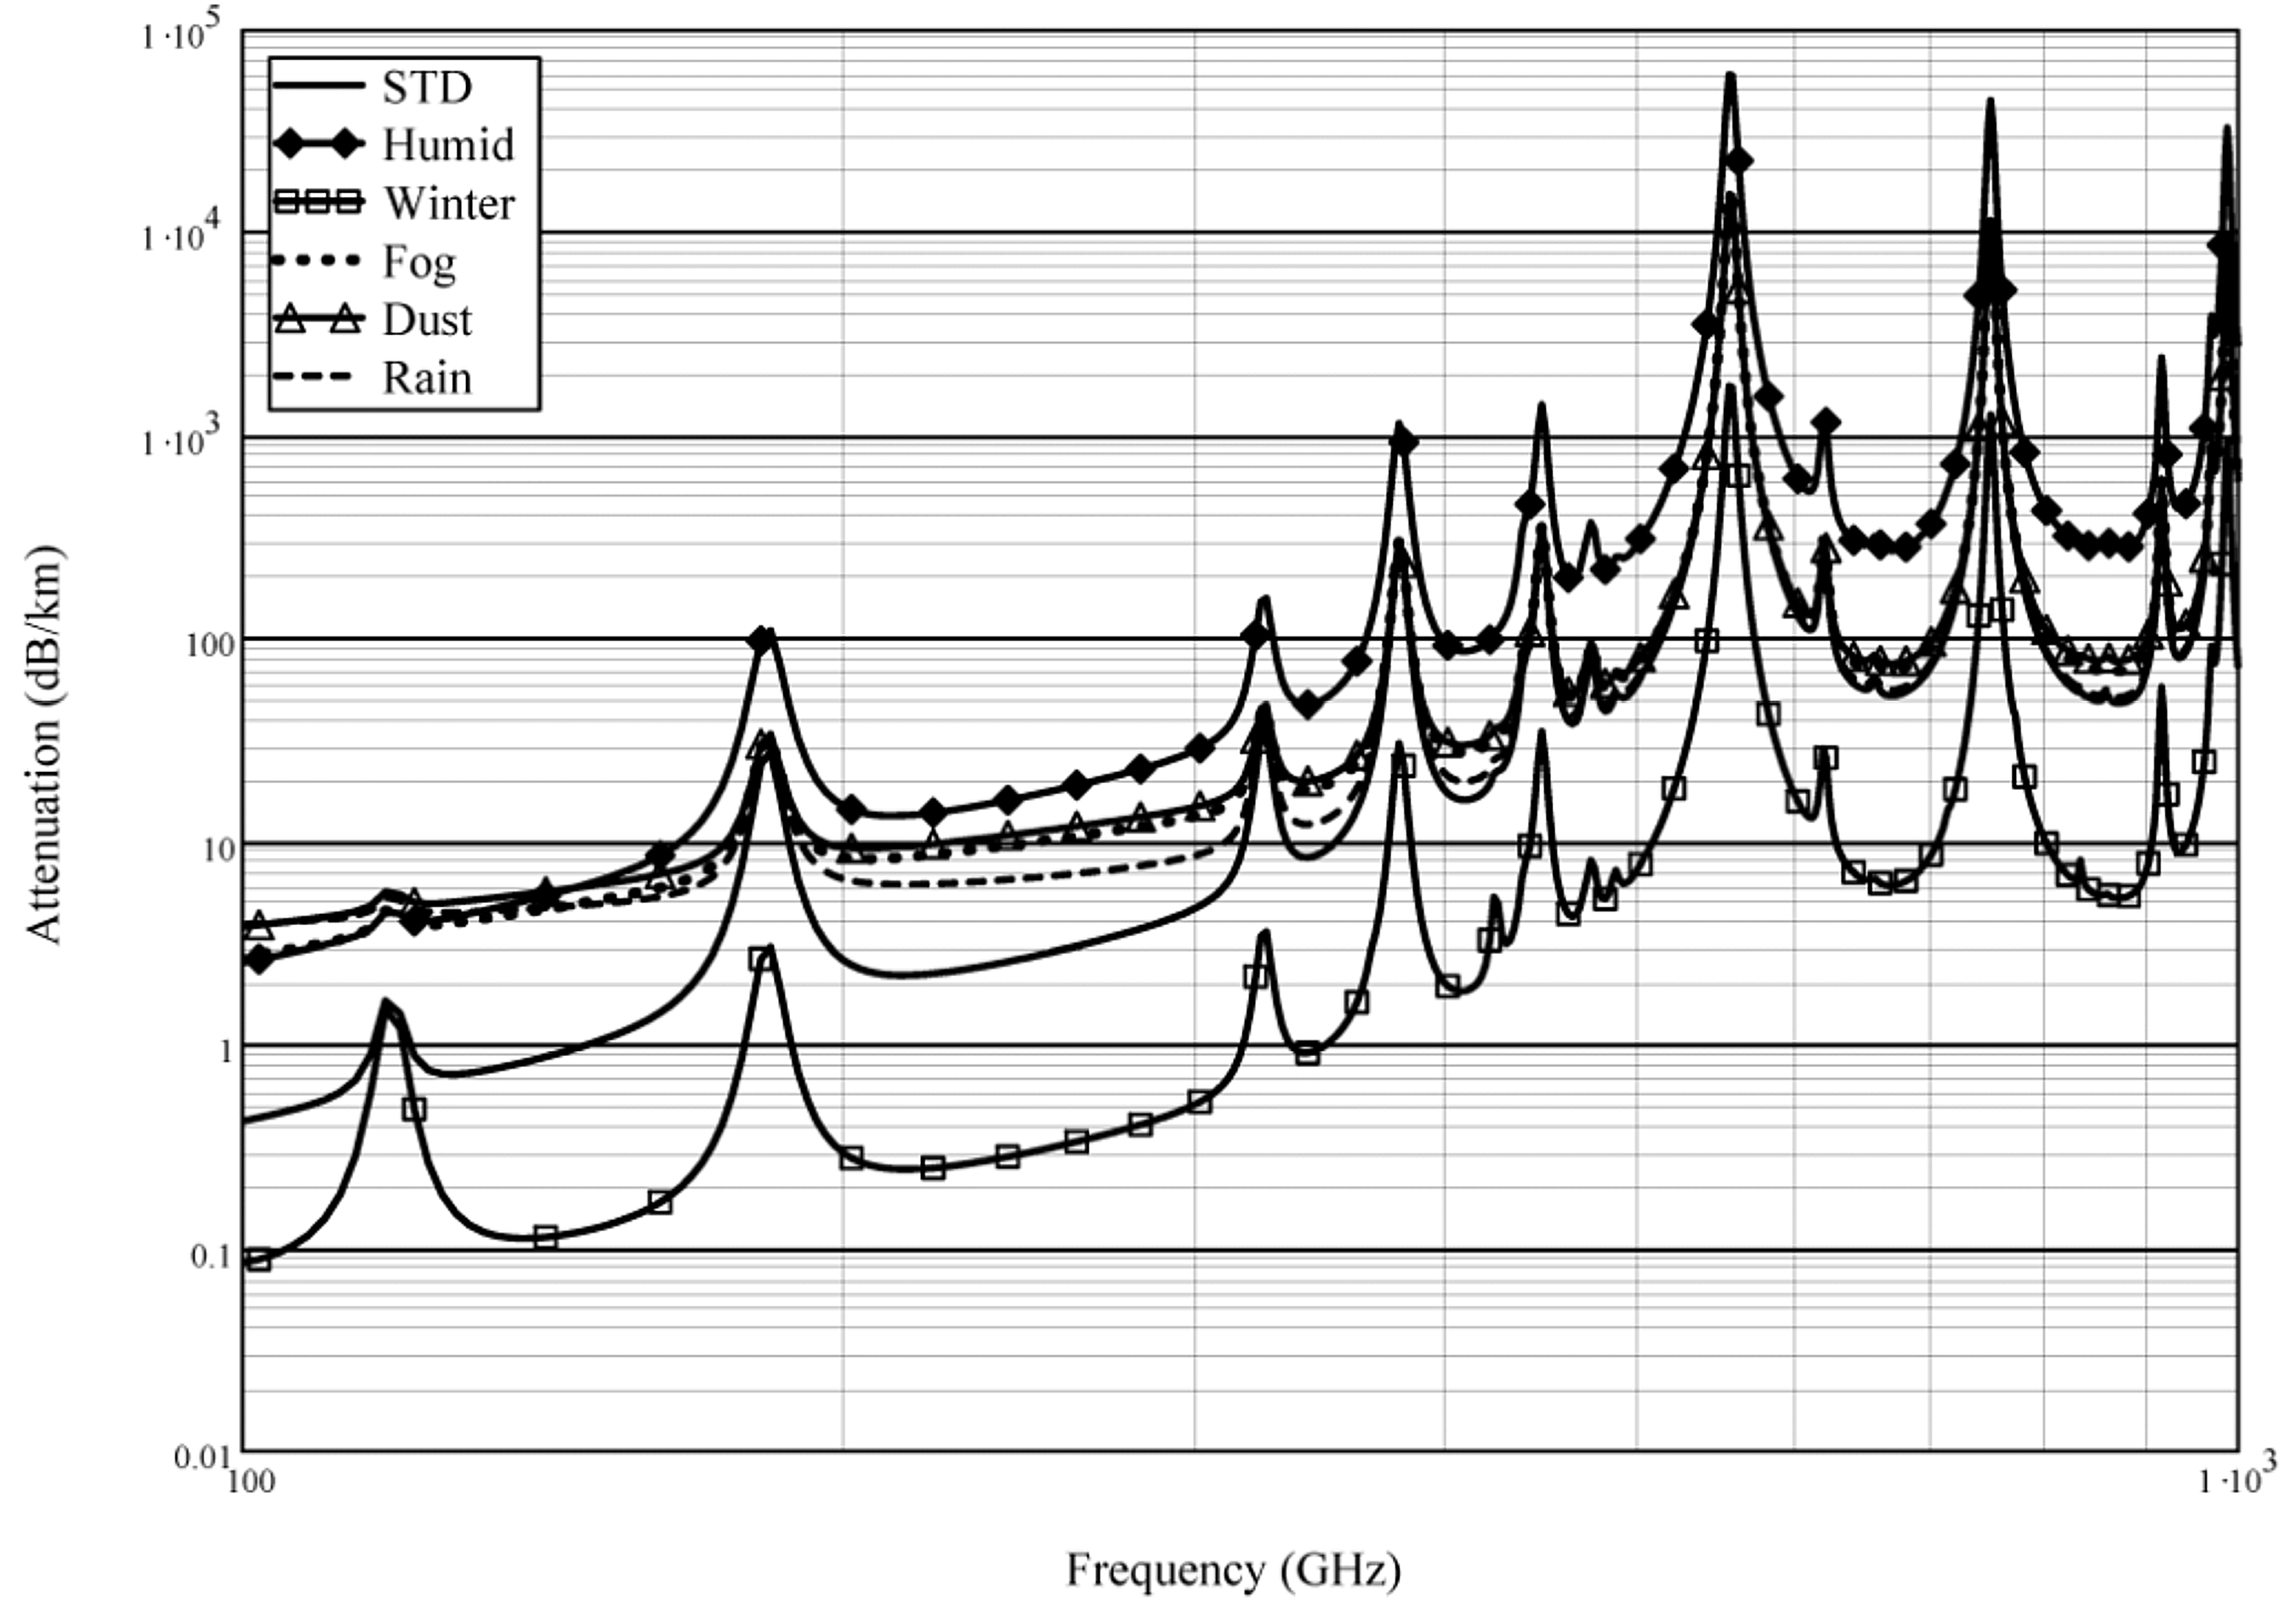
\includegraphics[width=4in]{../images/ch1-atmos-trans.png}};
    \begin{scope}[x={(image.south east)},y={(image.north west)}]
	    %\draw[help lines,xstep=.1,ystep=.1] (0,0) grid (1.0,1);
		%\foreach \x in {0,1,...,9} { \node [anchor=north] at (\x/10,0) {0.\x}; }
		%\foreach \y in {0,1,...,9} { \node [anchor=east] at (0,\y/10) {0.\y}; }
        
        % f = 100 GHz at 0.1055, f = 1000 GHz at 0.974.
        % 10 dB band is 318.0 -- 375.9 GHz
        % scale is logarithmic
		
        \draw[black,fill=blue!50,opacity=0.6] (0.5419, 0.099) rectangle (0.6050, 0.98) node[below right] {};
        
        \fill[fill=white] (0.0,0.00) rectangle (0.104,1.0);
        \fill[fill=white] (0.0,0.00) rectangle (1.0,0.095);
        \fill[fill=white] (0.98,0.08) rectangle (1.0,0.11);
        \node at (0.55,0.03) {Frequency (\si{\GHz})};
        \node at (0.105,0.05) {100};
        \node at (0.975,0.05) {1000};
        

        \node[rotate=90] at (-0.04,0.54) {Attenuation (dB/km)};
        \node[text width=1.4cm,align=flush right] at (0.02,0.10) {0.01};
        \node[text width=1.4cm,align=flush right]at (0.02,0.35) {1};
        \node[text width=1.4cm,align=flush right] at (0.02,0.6) {100};
        \node[text width=1.4cm,align=flush right] at (0.02,0.86) {10000};

        %\draw[black] (0.1055,0) -- (0.1055,1.00) node[midway,right] {}; % scale bar
        %\draw[black] (0.3669,0) -- (0.3669,1.00) node[midway,right] {}; % scale bar
        %\draw[black] (0.974,0) -- (0.974,1.00) node[midway,right] {}; % scale bar
    \end{scope}
\end{tikzpicture}

\end{document}
